
%(BEGIN_QUESTION)
% Copyright 2006, Tony R. Kuphaldt, released under the Creative Commons Attribution License (v 1.0)
% This means you may do almost anything with this work of mine, so long as you give me proper credit

Bestem følgende spenningsfall i denne nivåmålingskretsen når prosessnivået er 12 fot.  Merk at dette {\it ikke} er en loop-powered transmitter, men får strøm via separate kraftledere (120 volt AC).  Anta neglisjerbart (0) spenningsfall langs signallederlengdene:

$$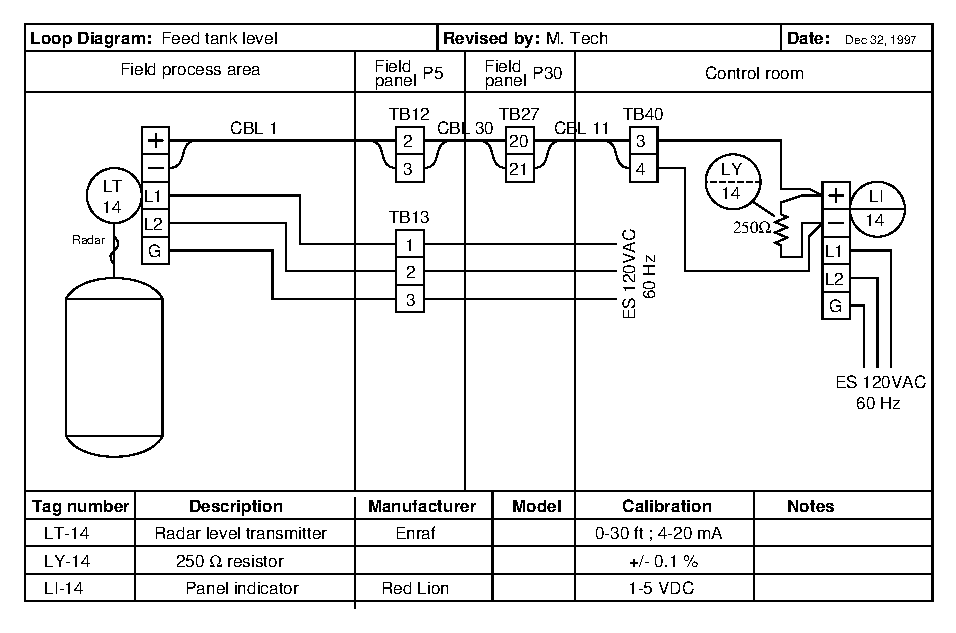
\includegraphics[width=15.5cm]{i00293x01.eps}$$

\begin{itemize}
\item{} Spenningsfall over transmitterens signalterminaler =
\item{} Spenningsfall mellom TB40-3 og TB27-21 =
\item{} Spenningsfall over 250 $\Omega$ motstand =
\item{} Spenningsfall mellom TB12-3 og TB27-21 =
\end{itemize}

\vskip 20pt \vbox{\hrule \hbox{\strut \vrule{} {\bf Forslag til sokratisk diskusjon} \vrule} \hrule}

\begin{itemize}
\item{} Demonstrer hvordan man kan {\it estimere} numeriske svar uten kalkulator.
\item{} Hvis spenningsfallet langs signalledningene var betydelig i stedet for null, hvordan ville spenningsberegningene blitt påvirket?  Ville betydelig sløyfemotstand gi nivåmålefeil?  Hvis ja, ville feilen blitt {\it høy} eller {\it lav}?
\item{} Forklar hvorfor akkurat denne nivåtransmitteren må være egenforsynt og ikke sløyfeforsynt, slik som er vanligere for prosesstransmittere.
\item{} Forklar hvorfor berøringsfrie radarnivåtransmittere må brukes bare på metalltanker for å oppfylle FCC-krav, mens guidet bølgeradar kan brukes på både metall- og ikke-metalltanker.
\item{} Når prosessnivået øker, vil spenningen over transmitterterminalene {\it øke}, {\it minke}, eller {\it forbli lik}?
\item{} Anta at denne egenforsynte (``4-wire'') nivåtransmitteren erstattes med en sløyfeforsynt (``2-wire'') transmitter.  Når prosessnivået øker, vil spenningen over transmitterterminalene {\it øke}, {\it minke}, eller {\it forbli lik}?
\end{itemize}

\underbar{file i00293}
%(END_QUESTION)





%(BEGIN_ANSWER)

\noindent
{\bf Delvis svar:}

\begin{itemize}
\item{} Spenningsfall over transmitterens signalterminaler =
\item{} Spenningsfall mellom TB40-3 og TB27-21 =
\item{} Spenningsfall over 250 $\Omega$ motstand = {\bf 2.6 volt}
\item{} Spenningsfall mellom TB12-3 og TB27-21 =
\end{itemize}

%(END_ANSWER)





%(BEGIN_NOTES)

En væskehøyde på 12 fot i et 0-30 fots område gir:

$${12 \hbox{ ft} \over 30 \hbox{ ft}} = 40\%$$

Disse 40\% tilsvarer et DC-signal på 10.4 mA til indikatoren, som gir 2.6 volt DC-fall over 250 $\Omega$ motstanden.

\begin{itemize}
\item{} Spenningsfall over transmitterterminaler = {\bf 2.6 volt}
\item{} Spenningsfall mellom TB40-3 og TB27-21 = {\bf 2.6 volt}
\item{} Spenningsfall over 250 $\Omega$ motstand = {\bf 2.6 volt}
\item{} Spenningsfall mellom TB12-3 og TB27-21 = {\bf 0 volt}
\end{itemize}

\vskip 20pt \vbox{\hrule \hbox{\strut \vrule{} {\bf Virtuell feilsøking} \vrule} \hrule}

Denne oppgaven egner seg godt til en ``virtuell feilsøking''-øvelse.  Presenter diagrammet for studentene, og bestem deg først for en konkret feil i systemet.  Presenter deretter ett eller flere symptomer på feilen (noe en operatør eller annen bruker ville kunne observere).  Studentene foreslår så diagnostiske tester for å identifisere type og plassering av feilen, som om de var teknikere som feilsøkte problemet.  Din jobb er å gi resultatene av hver foreslåtte test, og dokumentere dem slik at alle studentene ser dem.

Under og etter øvelsen er det nyttig å stille oppfølgingsspørsmål som:

\begin{itemize}
\item{} Hva forteller resultatet av siste diagnostiske test om feilen?
\item{} Anta at resultatet av siste diagnostiske test var annerledes.  Hva ville det i så fall fortalt om feilen?
\item{} Er siste diagnostiske test den beste testen vi kan gjøre?
\item{} Hva ville vært ideell testrekkefølge for å diagnostisere problemet på færrest mulig trinn?
\end{itemize}

%INDEX% Basics, line-powered transmitter: voltage drop calculations

%(END_NOTES)
